\documentclass[11pt,a4paper]{article}

\usepackage[utf8]{inputenc}
\usepackage[T1]{fontenc}
\usepackage[sc]{mathpazo}
\usepackage[scaled=0.9]{helvet}
\usepackage{courier}
\linespread{1.05}
\usepackage[margin=2.3cm]{geometry}
\usepackage{microtype}
\usepackage{xcolor}
\usepackage{enumitem}
\usepackage{booktabs}
\usepackage{tabularx}
\usepackage{array}
\usepackage{fancyhdr}
\usepackage{titlesec}
\usepackage{listings}
\usepackage{upquote}
\usepackage{needspace}
\usepackage{etoolbox}
\pretocmd{\section}{\Needspace*{9\baselineskip}}{}{}
\pretocmd{\subsection}{\Needspace*{6\baselineskip}}{}{}
\usepackage{amssymb}
\usepackage{tikz}
\usetikzlibrary{arrows.meta,positioning,fit,backgrounds}
\usepackage[most]{tcolorbox}
\usepackage[colorlinks=true,linkcolor=blue!50!black,urlcolor=blue!50!black]{hyperref}

\sloppy
\setlength{\parindent}{0pt}
\setlength{\parskip}{0.55em}
\setlist{itemsep=0.15em,topsep=0.25em,parsep=0pt}

% ---------- EDIT THESE ----------
\newcommand{\uid}{[HeUserID]}
\newcommand{\coursename}{[CS CRP]}
\newcommand{\duedate}{[23rd October, 2026]}
% --------------------------------

% Deliverable file names (single place to edit)
\newcommand{\dA}{\texttt{Deliverable\_1\_\allowbreak CONTEXT\_\allowbreak\uid.md}}
\newcommand{\dB}{\texttt{Deliverable\_2\_\allowbreak PLAN\_AND\_PROMPTS\_\allowbreak\uid.md}}
\newcommand{\dC}{\texttt{Deliverable\_3\_\allowbreak USER\_PROMPTS\_\allowbreak\uid.md}}
\newcommand{\dD}{\texttt{Deliverable\_4\_\allowbreak APP\_\allowbreak\uid.zip}}
\newcommand{\fn}[1]{\texttt{\detokenize{#1}}}

% ---------- Colours ----------
\definecolor{accent}{HTML}{1F4E79}
\definecolor{tipbg}{HTML}{EAF3FB}
\definecolor{warnbg}{HTML}{FDEDEC}
\definecolor{warnfg}{HTML}{A93226}
\definecolor{notebg}{HTML}{FEF9E7}
\definecolor{notefg}{HTML}{9A7D0A}

\titleformat{\section}{\Large\bfseries\color{accent}}{\thesection}{0.6em}{}[\vspace{-0.4em}\color{accent}\titlerule]
\titleformat{\subsection}{\large\bfseries\color{accent}}{\thesubsection}{0.6em}{}
\titleformat{\subsubsection}{\normalsize\bfseries}{\thesubsubsection}{0.6em}{}
\titlespacing*{\section}{0pt}{1.4em}{0.6em}
\titlespacing*{\subsection}{0pt}{1.0em}{0.4em}

\pagestyle{fancy}
\fancyhf{}
\fancyhead[L]{\small Homework 5 --- Context \& Prompt Engineering}
\fancyhead[R]{\small \coursename}
\fancyfoot[C]{\small Page \thepage}
\renewcommand{\headrulewidth}{0.3pt}

% ---------- Boxes ----------
\newtcolorbox{tipbox}[1][Tip]{enhanced,breakable,colback=tipbg,colframe=accent,
  fonttitle=\bfseries,title=#1,boxrule=0.6pt,arc=2pt,left=6pt,right=6pt,top=4pt,bottom=4pt}
\newtcolorbox{warnbox}[1][Warning]{enhanced,breakable,colback=warnbg,colframe=warnfg,
  fonttitle=\bfseries,title=#1,boxrule=0.6pt,arc=2pt,left=6pt,right=6pt,top=4pt,bottom=4pt}
\newtcolorbox{notebox}[1][Note]{enhanced,breakable,colback=notebg,colframe=notefg,
  fonttitle=\bfseries,title=#1,boxrule=0.6pt,arc=2pt,left=6pt,right=6pt,top=4pt,bottom=4pt}

% ---------- Listings ----------
\lstdefinestyle{code}{basicstyle=\ttfamily\footnotesize,breaklines=true,breakatwhitespace=false,
  frame=single,rulecolor=\color{black!35},backgroundcolor=\color{black!4},columns=fullflexible,
  keepspaces=true,showstringspaces=false,xleftmargin=2pt,xrightmargin=2pt,aboveskip=0.6em,belowskip=0.4em}
\lstset{style=code}

% ---------- Table helpers ----------
\newcolumntype{L}{>{\raggedright\arraybackslash}X}
\renewcommand{\arraystretch}{1.25}

\begin{document}

% =====================================================================
%  TITLE
% =====================================================================
\begin{tcolorbox}[enhanced,colback=accent,colframe=accent,coltext=white,arc=3pt,left=10pt,right=10pt,top=10pt,bottom=10pt]
{\Large\bfseries HOMEWORK 5}\\[2pt]
{\huge\bfseries Context Engineering, Prompt Engineering \& Multi-Agent ``Vibe Coding''}\\[6pt]
{\large Guided project: build a \emph{Research Paper Library \& Knowledge Graph} with a team of AI models}
\end{tcolorbox}

\begin{tabularx}{\textwidth}{@{}lXlX@{}}
\textbf{Course:} & \coursename & \textbf{Due:} & \duedate\\
\textbf{Type:} & Individual, guided project & \textbf{Submit:} & 4 files (see Section~\ref{sec:deliverables})\\
\end{tabularx}

\vspace{0.4em}
\begin{tcolorbox}[enhanced,breakable,colback=tipbg,colframe=accent,title=\bfseries Assignment at a glance,fonttitle=\bfseries,boxrule=0.6pt,arc=2pt]
\begin{itemize}
\item \textbf{Goal.} Learn how to get excellent software out of AI tools---even a \emph{weak} one---by giving it excellent \emph{context} and excellent \emph{prompts}.
\item \textbf{What you build.} A web app where you upload research-paper PDFs; it parses them, tags them, stores everything in SQLite, remembers who did what, and draws a knowledge graph connecting papers, authors and topics.
\item \textbf{How.} A fixed pipeline of free-tier AI tools: \textbf{Gemini Deep Research / DeepSeek} (research) $\rightarrow$ \textbf{Perplexity} (tech-stack lookup) $\rightarrow$ \textbf{Claude} (planning) $\rightarrow$ \textbf{Qwen 2.5 Coder 7B} (writes the whole app).
\item \textbf{Hard constraints.} Python + SQLite backend, vanilla HTML/CSS/JS frontend, \emph{no build step}, \emph{no Node.js/Bun/Deno}, \emph{no npm}, \emph{no JS frameworks}.
\item \textbf{You submit.} \dA, \\ \dB, \\ \dC\ and \\ \dD.
\item \textbf{Expected effort.} Roughly 10 hours spread over one weeks. Start early: free tiers have rate limits.
\end{itemize}
\end{tcolorbox}

\tableofcontents
\newpage

% =====================================================================
\section{Why This Assignment Exists}
% =====================================================================
Many people now build software by describing what they want to an AI and pasting the result back and forth---often called \textbf{vibe coding}. It feels magical for a 100-line game. It falls apart on anything with several files, a database and real-world messy input, because the AI is guessing about things you never told it.

The fix is not ``a smarter AI''. The fix is \textbf{you}, acting like a good engineering lead:
\begin{enumerate}
\item You \emph{investigate the problem domain} so you know what the input actually looks like. (\textbf{Context Engineering})
\item You \emph{write precise, structured instructions} so nothing is left to guess. (\textbf{Prompt Engineering})
\item You \emph{choose the right tool for each stage} instead of using one chatbot for everything. (\textbf{Multi-agent workflow})
\end{enumerate}

To prove the point, the last stage of this homework deliberately forces you to build the final app with a \textbf{small, weak model} (Qwen 2.5 Coder 7B). If your context and prompts are excellent, even this small model will produce a working app. If they are vague, it will visibly fail---and you will learn exactly why.

\subsection{Learning Objectives}
After this homework you should be able to:
\begin{enumerate}[label=\textbf{LO\arabic*.}]
\item Explain the difference between \emph{context engineering} and \emph{prompt engineering}, and when each applies.
\item Perform structured domain research and \emph{sift} it into a compact, machine-readable context pack.
\item Choose appropriate AI tools (research agents, search LLMs, reasoning models, coding models) for different project phases and justify the choice.
\item Select and verify a technology stack using up-to-date, citation-backed sources, avoiding deprecated libraries.
\item Write a complete architecture blueprint: file tree, database schema, API contract, build order.
\item Write verbose, deterministic prompts that a weak model can execute reliably, and debug failures systematically.
\item Respect real engineering constraints (no build step, fixed language/DB) and deliver a runnable, documented project.
\end{enumerate}

% =====================================================================
\section{Background: The Concepts You Must Understand}
% =====================================================================
Read this whole section before touching any AI tool. Your grade depends on applying these ideas, not just on the final app.

\subsection{Vibe Coding}
\textbf{Vibe coding} is a term popularized in early 2025 by Andrej Karpathy (former AI director at Tesla and OpenAI co-founder). The human stops writing code line by line and acts more like a product manager or director: describe the intent (``the vibe''), run the result, paste errors back, and let the AI write the code.

\textbf{The trap:} pure vibe coding collapses on multi-file projects into spaghetti code and endless bug loops, because the AI keeps forgetting or inventing details. The cure is the two disciplines below.

\subsection{Chatbot vs.\ AI Agent}
\begin{tabularx}{\textwidth}{@{}>{\bfseries}p{2.6cm}L L@{}}
\toprule
 & \textbf{Chatbot (conversational LLM)} & \textbf{AI agent (agentic coding system)}\\
\midrule
What it is & A passive, turn-based interface: you send text, it returns text. Examples: web chat UIs of Claude, Gemini, DeepSeek, Perplexity, Qwen. & An LLM connected to \emph{tools, memory and an execution environment}. Examples: Cursor/Windsurf (agent mode), Cline, Claude Code, GitHub Copilot agent features.\\
Can it touch your files? & No. You copy and paste. & Yes: reads your folder, edits many files, runs terminal commands.\\
Can it check its own work? & No. It cannot run its code. & Yes: runs the code, reads the error, fixes it in a loop.\\
In this homework & Most of your tools are chatbots (or search/research agents). \emph{You} are the execution environment: you run the code and report errors. & Research tools such as Deep Research behave agent-like (they browse autonomously), but coding is done through chat.\\
\bottomrule
\end{tabularx}

\begin{notebox}[Terminology note]
``GPT'' (Generative Pre-trained Transformer) is OpenAI's product branding. The correct umbrella term for DeepSeek, Gemini, Claude, Qwen and similar systems is \textbf{LLM (Large Language Model)}. Models that deliberately ``think'' step by step before answering are often called \textbf{reasoning models}.
\end{notebox}

\subsection{Tokens and the Context Window}
\begin{itemize}
\item \textbf{Token:} the unit of text an LLM reads and writes. Roughly 1 token $\approx$ 4 characters $\approx$ 0.75 English words.
\item \textbf{Context window:} the model's working memory for \emph{one session}: your prompt, attached files, the whole chat history \emph{and} the model's own replies must all fit inside it.
\item \textbf{Different models, very different windows.} Gemini's long-context models are at the top of the public range (hundreds of thousands up to around a million tokens or more, depending on the version and where you use it, e.g.\ Google AI Studio). DeepSeek's chat models are in the tens-to-low-hundreds of thousands. Free web tiers often cap you well below a model's advertised maximum. Small models such as Qwen 2.5 Coder 7B may have large advertised limits, but in practice (especially when run locally or via free hosts) you should treat them as having a \emph{small effective window} and keep every prompt short and focused.
\item \textbf{Context rot / ``lost in the middle'':} the more irrelevant material you pour in, the worse the model attends to your actual instructions. Instructions buried in the middle of a huge prompt are the first to be ignored. \emph{More context is not better context.}
\end{itemize}

\subsection{Context Engineering}
\begin{tcolorbox}[colback=white,colframe=accent,boxrule=0.6pt,arc=2pt]
\textbf{Definition.} Context engineering is the systematic practice of \emph{curating, structuring, compressing and sequencing} the information placed in an LLM's context window---domain rules, documentation, data schemas, examples, file trees, constraints---so that the model can reason accurately instead of guessing.
\end{tcolorbox}

\textbf{Analogy.} If prompt engineering is \emph{how you phrase the question}, context engineering is \emph{the open-book study guide you hand over before asking it}.

\textbf{Why you can't skip it.} You cannot design an algorithm or a tool without knowing what its \emph{input} looks like. A program that ingests research papers must be designed around how research papers are actually structured, how PDFs actually store text, and how citations are actually written. If you don't know these things, neither does the AI---it will invent plausible nonsense (a \emph{hallucination}).

\textbf{The four pillars}
\begin{enumerate}
\item \textbf{Discovery \& retrieval.} Gather raw domain truth: what is in a research paper? How are PDFs built? Which free APIs return clean metadata? Which Python libraries parse PDFs well? (Tools: Gemini Deep Research, DeepSeek, Perplexity.)
\item \textbf{Selection \& pruning (sifting).} Throw away fluff, history, marketing, and irrelevant edge cases. Keep only what changes a design or coding decision.
\item \textbf{Structuring.} Convert messy notes into clean, machine-readable reference material: Markdown specs, JSON examples, SQL schemas, tables, short code snippets.
\item \textbf{State management.} Maintain a small ``memory bank'' (your \fn{CONTEXT.md}, architecture notes, a running ``what is done / what is next'' list) that you paste at the start of each new AI session so it instantly knows the project's state.
\end{enumerate}

\subsection{Prompt Engineering}
\begin{tcolorbox}[colback=white,colframe=accent,boxrule=0.6pt,arc=2pt]
\textbf{Definition.} Prompt engineering is the tactical craft of structuring instructions, roles, constraints and output formats so an LLM produces a predictable, high-quality result.
\end{tcolorbox}

\textbf{Analogy.} Once the AI has the background (context), the prompt is the \emph{work order or ticket}. A great ticket leaves zero room for guessing.

\textbf{Anatomy of a good engineering prompt}
\begin{enumerate}
\item \textbf{Role \& objective} --- \emph{``You are a senior Python backend engineer. Write the PDF ingestion module.''}
\item \textbf{Context reference} --- the exact facts needed (pasted in, since most chat tools cannot read your files): schema, API contract, sample input/output.
\item \textbf{Tech stack \& constraints} --- exact language version, libraries, and prohibitions (\emph{``Do NOT use PyPDF2; do NOT use Node or npm''}).
\item \textbf{Interface contract} --- exact file name, function signatures, input and output types.
\item \textbf{Step-by-step plan} --- numbered steps the model should follow.
\item \textbf{Output format} --- \emph{``Return only the complete contents of \fn{parser.py} in one code block. No explanation.''}
\item \textbf{(Optional) Examples} --- one small input and the exact expected output (few-shot).
\end{enumerate}

\subsection{Context Engineering vs.\ Prompt Engineering}
\begin{tabularx}{\textwidth}{@{}>{\bfseries}p{3.1cm}LL@{}}
\toprule
\textbf{Dimension} & \textbf{Context engineering (the environment)} & \textbf{Prompt engineering (the command)}\\
\midrule
Core question & ``What does the AI need to \emph{know} to do this job?'' & ``What exact \emph{task} do I want it to do right now?''\\
Project phase & Research, discovery, architecture setup & Active coding, debugging, iteration\\
Typical artifacts & Domain notes, API docs, schemas, sample files, constraint lists & Step-by-step instructions, contracts, output-format rules, examples\\
If you skip it & \textbf{Hallucination:} fake libraries, wrong assumptions about input, broken integrations & \textbf{Ambiguity:} wrong language, sloppy or partial code, vague answers\\
\bottomrule
\end{tabularx}

\subsection{Why We Force a Weak Model at the End}
A frontier model can often recover from a vague prompt by guessing correctly. A 7B-parameter model cannot. That makes it an excellent \emph{measuring instrument}: if Qwen 2.5 Coder 7B builds your app, it is because your context and prompts were good. Expect to learn these habits the hard way:
\begin{itemize}
\item One small task per prompt; one file (or even one function) at a time.
\item State the exact interface (names, parameters, return types) so independently generated files fit together.
\item Paste only the context \emph{relevant to that task}, not your whole research.
\item Re-state the hard constraints in every prompt; small models forget them.
\item Start a \emph{fresh chat} when the conversation gets long or the model starts to drift.
\end{itemize}

% =====================================================================
\clearpage
\section{The Tool Landscape and Your Assigned Roles}
% =====================================================================
Different AI tools are good at different jobs. This homework assigns a tool to each phase. Use the assigned tools; the point is to learn \emph{why} each fits its role.

\begin{tabularx}{\textwidth}{@{}>{\raggedright\arraybackslash}p{2.5cm}LLL@{}}
\toprule
\textbf{Tool} & \textbf{Strengths} & \textbf{Weaknesses} & \textbf{Role in this homework}\\
\midrule
\textbf{Gemini} (Deep Research; long-context models) & Browses the web autonomously and compiles long cited reports. Very large context window: can read many PDFs at once. & Can over-engineer if not constrained. Free-tier Deep Research usage is limited. & \textbf{Phase 1:} domain research; digesting sample papers.\\
\textbf{DeepSeek} (chat, with reasoning mode) & Free; strong step-by-step reasoning for logic, algorithms and architecture. & Slow, because it \emph{thinks} before answering (not because of memory). Smaller window than Gemini. Servers are sometimes busy. & \textbf{Phase 1:} alternative or complement to Gemini for research and reasoning.\\
\textbf{Perplexity} & Fast, citation-backed lookups of current library versions, APIs and documentation. & Small context; poor at writing large multi-file code. & \textbf{Phase 2:} choosing libraries and checking they are current and not deprecated.\\
\textbf{Claude} (free tier) & Excellent at structured, well-organized, detailed writing and planning. & Free tier has a small message/token budget that runs out quickly. & \textbf{Phase 3:} turn your context and stack into the full plan and prompts. \emph{Do not waste it on research.}\\
\textbf{Qwen 2.5 Coder 7B} (Alibaba; free tier or local) & Free, code-specialized, surprisingly capable when given precise instructions. & Small model: forgets constraints, weak at long reasoning, easily confused by vague prompts. & \textbf{Phase 4 (mandatory):} writes \emph{all} application code.\\
\bottomrule
\end{tabularx}

\begin{warnbox}[Tool usage rules]
\begin{itemize}
\item \textbf{Do not use Claude in Phase 1 or Phase 2.} Its free-tier budget is limited; save it for planning.
\item \textbf{All application code must come from Qwen 2.5 Coder 7B (Instruct variant).} Do not use Claude, ChatGPT, Gemini, Copilot or any other model to write or fix application code. (Manual edits are allowed in a limited, logged form; see Section~\ref{sec:phase4}.)
\item Free tiers, model names and limits change often. If an assigned tool is unavailable to you, tell the instructor \emph{before} substituting, and record the substitution in \dC.
\item You may run Qwen through a free hosted chat/API provider, or locally (for example with Ollama: \fn{ollama run qwen2.5-coder:7b}, or LM Studio) if your laptop can handle a 7B model. Record which route you used and the exact model name.
\end{itemize}
\end{warnbox}

% =====================================================================
\section{The Project: Research Paper Library \& Knowledge Graph}
% =====================================================================
\subsection{The Idea}
You are building a personal \textbf{digital library for research papers}. A user uploads a paper as a PDF. The app:
\begin{enumerate}
\item parses it and extracts the title, authors, abstract, keywords, references and other useful metadata;
\item automatically assigns \textbf{tags} and \textbf{subject matters} (topics);
\item stores everything in a \textbf{SQLite} database, including a record of \emph{who uploaded or changed what, and when};
\item lets the user browse and search the library;
\item as more papers are added, draws an interactive \textbf{knowledge graph} in which papers, authors and topics are connected to each other.
\end{enumerate}

\subsection{Why This Is a Perfect Context-Engineering Exercise}
If you simply tell an AI ``make an app that reads PDFs and graphs them'', it will fail. PDFs are not structured documents like HTML or Word; they are drawing instructions that place glyphs at coordinates on a page. Academic papers add more difficulty: two-column layouts, headers and footers, equations, ligatures, hyphenated line breaks, and many different citation styles. Before you can design \emph{any} parser you must understand what a research paper looks like from the inside. That is your Phase~1 research.

\subsection{Functional Requirements}
\begin{tabularx}{\textwidth}{@{}>{\bfseries}p{1cm}L p{2.2cm}@{}}
\toprule
\textbf{ID} & \textbf{Requirement} & \textbf{Priority}\\
\midrule
F1 & Upload a PDF through the browser; the file is stored on the server and a record is created. & Must\\
F2 & Parse the PDF and extract at least: title, author list, abstract. Extract keywords, DOI/arXiv ID, year and venue where available. & Must\\
F3 & Extract the reference list and store each reference as a separate record (raw text at minimum; structured fields if you can). & Must\\
F4 & Automatically assign tags/subjects to each paper (see ideas in Section~\ref{sec:phase1}). Tags must be stored in the database. & Must\\
F5 & Persist everything in SQLite with sensible relational tables (papers, authors, topics, references, links between them). & Must\\
F6 & Record who did what: every upload, edit, tag change and deletion is logged with a user name, action and timestamp. A simple ``enter your name'' or minimal registration is sufficient; full password security is not required. & Must\\
F7 & Library view: list papers, search/filter by title, author, topic or tag. & Must\\
F8 & Paper detail view: show the extracted metadata, abstract, tags and references; allow correcting metadata by hand. & Should\\
F9 & Knowledge graph view: interactive graph with at least three node types (paper, author, topic) and meaningful edges. It must update as papers are added. & Must\\
F10 & Activity/history view: show the log from F6. & Should\\
F11 & Delete a paper (and keep the graph and database consistent). & Should\\
F12 & Handle bad input gracefully: non-PDF files, scanned PDFs without text, duplicate uploads. Show clear error messages instead of crashing. & Should\\
\bottomrule
\end{tabularx}

\subsection{The Graph Model}
Your research and plan must make these concepts precise. A starting point:
\begin{itemize}
\item \textbf{Nodes:} \emph{Paper}, \emph{Author}, \emph{Topic} (optionally \emph{Venue} or \emph{Keyword}).
\item \textbf{Edges:} \fn{AUTHORED_BY} (paper--author), \fn{HAS_TOPIC} (paper--topic), \fn{CITES} (paper--paper, only when the cited paper is also in the library), and derived edges such as \fn{CO_AUTHOR} (author--author) and \fn{RELATED_TOPIC} (topic--topic, e.g.\ topics that co-occur in the same papers).
\item \textbf{Design question to answer:} Do you store the edges in tables, or compute them from existing tables when the graph is requested? Justify your choice in \dB.
\end{itemize}

\begin{tipbox}[Hint: don't parse everything from the PDF alone]
Messy PDF text is a fragile source of truth. A smart engineer extracts a stable identifier (a DOI or arXiv ID, or at worst a clean title) and asks a free scholarly metadata service for \emph{clean JSON} (for example Crossref, Semantic Scholar, OpenAlex or the arXiv API). Investigate these services in Phase~1: what do they return, what are their rate limits and licensing terms, and what happens when a paper has no DOI? Your app should still work (in a degraded way) when the network or the lookup fails.
\end{tipbox}

% =====================================================================
\section{Hard Constraints (Non-Negotiable)}
\label{sec:constraints}
% =====================================================================
\begin{warnbox}[Violating any of these costs you heavily (see grading)]
These apply to the \emph{final app}. Re-state them in every prompt you give to Claude and Qwen.
\end{warnbox}

\subsection{Overall}
\begin{itemize}
\item The project must be \textbf{web-based}.
\item \textbf{Backend language: Python.} \textbf{Database: SQLite.} You may use any number of Python libraries (installed with \fn{pip} and listed in \fn{requirements.txt}).
\item \textbf{No build process} for the frontend \emph{or} the backend.
\item \textbf{Strictly forbidden:} Node.js, Bun, Deno, and any JavaScript backend; \fn{npm} (and \fn{yarn}, \fn{pnpm}); any \fn{package.json} or \fn{node_modules} in your project.
\end{itemize}

\subsection{Strict Frontend Constraints (No-Build Architecture)}
\begin{enumerate}
\item \textbf{Environment:} browser-native client-side code only: HTML5, CSS3 and vanilla ES6+ JavaScript.
\item \textbf{No Node.js:} do not generate a \fn{package.json}; do not use \fn{npm} or \fn{node_modules}; do not use build tools (no Vite, Webpack, Babel or TypeScript).
\item \textbf{No frameworks:} no React, Vue, Angular or JSX. Manipulate the DOM directly with standard Web APIs (\fn{document.querySelector}, \fn{fetch}, etc.).
\item \textbf{External libraries via CDN only:} if you need third-party libraries (for example \fn{vis-network} or \fn{cytoscape} for graphs, \fn{pdf.js} for PDFs), load them strictly through \fn{<script src="https://cdn.jsdelivr.net/...">} tags in \fn{index.html}, or through browser-native ES-module URL imports (\fn{import ... from 'https://esm.sh/...'}).
\item \textbf{Execution:} the frontend must work immediately when opened through a static file server or directly from \fn{index.html}.
\end{enumerate}

\begin{notebox}[Engineering detail you should research: serving and CORS]
If your page is opened straight from disk (\fn{file://}) and calls your Python server with \fn{fetch}, the browser will block the request unless the backend sends CORS headers. If instead your Python server also serves the static frontend files, there is no CORS problem. Decide which approach you use, say so in your plan, and make sure the app works with the exact instructions in your README. Also pin your CDN library versions in the URLs so the app does not break when a library updates.
\end{notebox}

\subsection{Quick Self-Check Before Submitting}
\begin{lstlisting}
# From the project root (inside the unzipped folder), these must find nothing:
find . -name package.json -o -name node_modules -o -name "*.jsx" -o -name "*.tsx" -o -name "*.ts"
grep -rniE "from 'react'|require\(|webpack|vite|babel" --include=*.js --include=*.html .
\end{lstlisting}

% =====================================================================
\section{The Workflow: Four Phases, Four Tools}
\label{sec:workflow}
% =====================================================================
\begin{center}
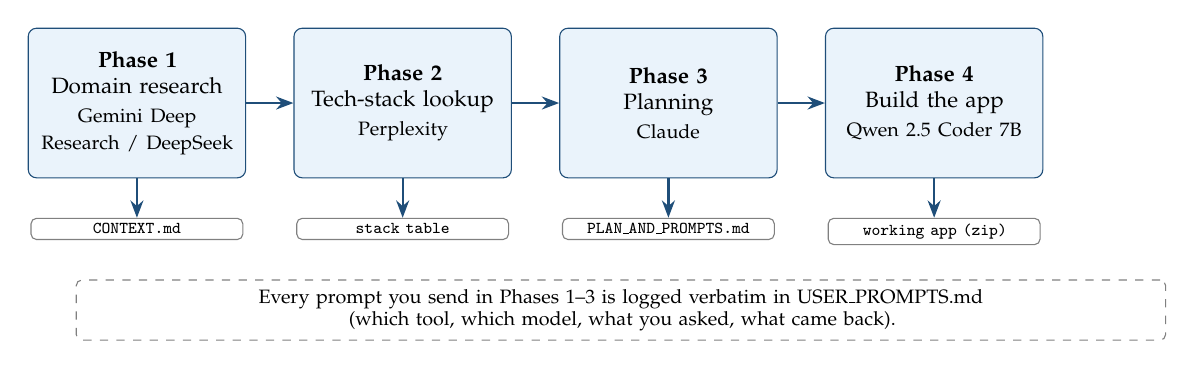
\begin{tikzpicture}[
  box/.style={draw=accent,fill=tipbg,rounded corners=3pt,text width=2.55cm,align=center,minimum height=1.9cm,font=\footnotesize,inner sep=3pt},
  outb/.style={draw=black!50,fill=white,rounded corners=2pt,text width=2.55cm,align=center,font=\fontsize{6.5}{7.5}\selectfont\ttfamily,inner sep=2pt},
  arr/.style={-{Stealth[length=2.2mm]},thick,accent},
  node distance=6mm]
\node[box] (p1) {\textbf{Phase 1}\\Domain research\\[1pt]{\scriptsize Gemini Deep Research / DeepSeek}};
\node[box,right=of p1] (p2) {\textbf{Phase 2}\\Tech-stack lookup\\[1pt]{\scriptsize Perplexity}};
\node[box,right=of p2] (p3) {\textbf{Phase 3}\\Planning\\[1pt]{\scriptsize Claude}};
\node[box,right=of p3] (p4) {\textbf{Phase 4}\\Build the app\\[1pt]{\scriptsize Qwen 2.5 Coder 7B}};
\node[outb,below=5mm of p1] (o1) {CONTEXT.md};
\node[outb,below=5mm of p2] (o2) {stack table};
\node[outb,below=5mm of p3] (o3) {PLAN\_AND\_PROMPTS.md};
\node[outb,below=5mm of p4] (o4) {working app (zip)};
\draw[arr] (p1) -- (p2);
\draw[arr] (p2) -- (p3);
\draw[arr] (p3) -- (p4);
\foreach \i in {1,2,3,4} \draw[arr] (p\i) -- (o\i);
\node[draw=black!50,dashed,rounded corners=2pt,font=\scriptsize,text width=13.6cm,align=center,below=5mm of o2.south west,anchor=north west,xshift=-2.8cm] (log) {Every prompt you send in Phases 1--3 is logged verbatim in USER\_PROMPTS.md (which tool, which model, what you asked, what came back).};
\end{tikzpicture}
\end{center}

\begin{tipbox}[The golden rule of this pipeline]
\textbf{The output of each phase is the input of the next.} Do not paste raw chat transcripts forward; paste a \emph{cleaned, structured artifact}. Quality compounds: good context $\rightarrow$ good plan $\rightarrow$ good prompts $\rightarrow$ working code.
\end{tipbox}

% ---------------------------------------------------------------------
\subsection{Phase 1 --- Domain Research and Context Engineering}
\label{sec:phase1}
% ---------------------------------------------------------------------
\textbf{Goal:} understand the \emph{input} (research-paper PDFs) and the \emph{ecosystem} (libraries, APIs, techniques) well enough that you could explain exactly what the program must do. \textbf{Tools:} Gemini Deep Research and/or DeepSeek. \textbf{Output:} \dA.

\subsubsection{Step 1: Ask the right questions}
Do not ask one giant question like ``how do I build this app?''. Run several focused research sessions. Your research must at least answer the following.

\begin{enumerate}[label=\textbf{Q\arabic*.}]
\item \textbf{Anatomy of a research paper.} Which sections exist, in what order, and what do they contain (title block, authors and affiliations, abstract, keywords, introduction, methods, results, discussion, conclusion, acknowledgements, references)? How do conference papers, journal papers and arXiv preprints differ?
\item \textbf{The PDF problem.} How does a PDF actually store text? Why do two-column layouts, headers/footers, footnotes, equations, ligatures and hyphenation break naive text extraction? What is the difference between a text PDF and a scanned PDF?
\item \textbf{Citation and reference styles.} What do IEEE (numbered), APA, MLA, Chicago and BibTeX-style references look like? How are in-text citations different from the bibliography? Give a \emph{real} example of each.
\item \textbf{Identifiers and metadata services.} What are a DOI and an arXiv ID, what do they look like (patterns), and where do they appear in a PDF? Which free scholarly APIs can turn them into clean metadata? What fields do they return, and what are the rate limits and terms?
\item \textbf{Extraction techniques.} Which Python libraries extract text and layout from PDFs (and what are their trade-offs)? Which approaches find the title, authors, abstract and reference section (heuristics such as font size and position, regular expressions, section-heading detection, metadata lookup, or an LLM)?
\item \textbf{Tagging and topic assignment.} Which techniques can assign keywords/topics automatically using only free and local tools (for example keyword extraction such as RAKE/YAKE/TF--IDF, using the paper's own keywords, matching against a small controlled vocabulary, or topic information returned by a scholarly API)? What are the strengths and limits of each?
\item \textbf{Knowledge graphs.} What is a graph in the data-structure sense (nodes, edges, directed vs.\ undirected)? How do you represent one in relational tables? Which browser libraries draw interactive graphs from a CDN, and what JSON format do they expect?
\item \textbf{Edge cases.} What goes wrong in real papers: missing abstract, multi-line titles, many authors, non-English text, no DOI, scanned pages, references split across columns, duplicate uploads?
\end{enumerate}

\subsubsection{Step 2: Choose and use the right research tool}
\begin{itemize}
\item \textbf{Gemini Deep Research}: give it a clear, scoped brief. It browses many sources and returns a long cited report. Check the citations; do not trust every claim.
\item \textbf{DeepSeek}: use it to reason through design questions, compare approaches, and cross-check Gemini's report. Expect slower answers.
\item \textbf{Use both when possible} and compare. Where they disagree, find out which is right. Noting a disagreement you resolved is a mark of strong research.
\end{itemize}

\begin{tipbox}[Starter research prompt (adapt it; do not copy it blindly)]
\begin{lstlisting}[frame=none,backgroundcolor=\color{white},xleftmargin=0pt]
I am designing a program that ingests academic research papers as PDF
files and extracts structured metadata (title, authors, abstract,
keywords, references). I have not yet chosen any design. Research and
report on: (1) the typical structure of conference, journal and arXiv
papers; (2) why PDF text extraction is hard for two-column papers and
how Python libraries handle it; (3) the main citation styles with one
real example each; (4) DOI and arXiv ID formats and free metadata APIs
with their response fields and rate limits. Cite every source. Prefer
concrete examples and short sample JSON over general prose.
\end{lstlisting}
\end{tipbox}

\subsubsection{Step 3: Sift (the heart of context engineering)}
Raw research reports are long, repetitive and full of noise. Your job is to compress them into what the downstream AI actually needs.

\begin{tabularx}{\textwidth}{@{}LL@{}}
\toprule
\textbf{Keep (changes a design or code decision)} & \textbf{Throw away (noise)}\\
\midrule
Concrete formats, patterns and examples (regexes for DOI, a real IEEE reference line, a real API JSON response, trimmed) & History of the PDF format, publishing-industry politics, marketing language\\
Library names with a one-line trade-off each & Long tutorials, installation walk-throughs, unrelated libraries\\
Edge cases that will actually break your parser & Exotic cases outside your scope (e.g.\ training your own OCR model)\\
Precise definitions of your graph's nodes and edges & Generic explanations of what a graph is\\
Sources (URLs) so claims can be re-checked & Unsourced claims you could not verify\\
\bottomrule
\end{tabularx}

Aim for a context pack small enough to paste into a model with a modest window \emph{together with} other instructions: roughly \textbf{1\,500 to 3\,500 words}, dense and well structured. In \dA, include a short ``\textbf{What I discarded and why}'' section; this shows your sifting judgement.

\subsubsection{Step 4 (bonus): Ground your research in real samples}
\textbf{Extra credit.} Download \textbf{three to five real research papers} (open-access ones: for instance from arXiv; choose a mix, e.g.\ one two-column conference paper, one single-column paper, one with many authors). Give them to Gemini (it can ingest several PDFs at once) and ask it to extract the title, authors, abstract and references, and to describe the exact patterns it sees (where the DOI appears, how the reference section starts, how references are numbered). Put the \emph{observed} patterns and a few short, real excerpts into your context pack. Real samples beat imagination; this is the single best way to stop the coding model from hallucinating about the input. Evidence of this step (the prompt, the sample list, and the findings) is required to receive the bonus.

\begin{warnbox}[Respect copyright]
Use papers you may legally download (open access/preprints). In your submission include only short excerpts needed for illustration, not whole papers.
\end{warnbox}

\subsubsection{Required content of \dA}
\begin{lstlisting}
# CONTEXT - Research Paper Library & Knowledge Graph
## 1. Project in one paragraph
## 2. Anatomy of a research paper (sections, order, what each contains)
## 3. The PDF problem (how text is stored; two-column, scanned, etc.)
## 4. Citation styles (IEEE / APA / MLA / BibTeX) - one REAL example each
## 5. Identifiers and metadata APIs
   - DOI / arXiv ID patterns and where they appear
   - For each API: endpoint, auth, rate limit, trimmed sample JSON
## 6. Extraction techniques considered -> which one I chose and why
## 7. Tagging / topic assignment techniques -> chosen approach
## 8. Knowledge-graph model (nodes, edges, direction, derived edges)
## 9. Edge cases and failure modes the app must handle
## 10. Sample-paper findings (bonus, if done)
## 11. What I discarded and why (sifting log)
## 12. Sources (URLs)
\end{lstlisting}

% ---------------------------------------------------------------------
\subsection{Phase 2 --- Technology-Stack Lookup}
\label{sec:phase2}
% ---------------------------------------------------------------------
\textbf{Goal:} pick specific, \emph{current}, non-deprecated libraries for each need and record exact versions. \textbf{Tool:} Perplexity. \textbf{Output:} the technology table that goes into \dB.

\textbf{Why Perplexity?} Coding models are trained on data that is months or years old, so they happily use functions that have been renamed, deprecated or removed. Perplexity answers with live web sources and citations, which makes it ideal for ``is this library still maintained, and what is its current API?'' (It has a small effective context, so use it for short, targeted lookups only---not for generating your project.)

\textbf{What to look up.} For each row, ask a precise question, open the cited source, and confirm it yourself:
\begin{center}
\begin{tabularx}{\textwidth}{@{}p{3.6cm}L@{}}
\toprule
\textbf{Need} & \textbf{Questions to answer}\\
\midrule
Python web framework & Which lightweight framework (e.g.\ Flask, FastAPI, or another) fits a small app that also serves static files and accepts file uploads? Current stable version? Any upload or CORS gotchas?\\
PDF text/layout extraction & Which actively maintained library (e.g.\ PyMuPDF, pdfplumber, pypdf) best handles two-column papers? Is any option deprecated or unmaintained (e.g.\ PyPDF2)?\\
Metadata extraction / APIs & Which HTTP client library? Current endpoint and response format for Crossref / Semantic Scholar / OpenAlex / arXiv? Rate limits?\\
Tagging / keyword extraction & Which Python library (if any) for local keyword extraction? Is it maintained? Does it need big model downloads?\\
SQLite access & Use the standard-library \fn{sqlite3} or an ORM? What is the recommended way to avoid SQL injection?\\
Graph visualization (CDN) & Current stable version of \fn{vis-network}, \fn{cytoscape.js} or similar; the exact jsDelivr URL; the required data format; does it need an extra CSS file?\\
\bottomrule
\end{tabularx}
\end{center}

\textbf{Record for each choice:} library name, \textbf{exact version}, purpose, why chosen over alternatives, and the \textbf{source URL}. Prefer official documentation or package-index pages over blog posts.

\begin{tipbox}[Example lookup prompt]
\begin{lstlisting}[frame=none,backgroundcolor=\color{white},xleftmargin=0pt]
What is the current stable version of PyMuPDF, and what is the
recommended way to extract text blocks with positions from a PDF page
in Python? Is PyPDF2 deprecated? Cite the official documentation.
\end{lstlisting}
\end{tipbox}

% ---------------------------------------------------------------------
\subsection{Phase 3 --- Planning and Prompt Writing with Claude}
\label{sec:phase3}
% ---------------------------------------------------------------------
\textbf{Goal:} turn your context pack and stack table into a complete blueprint---detailed enough that a 7B model can build the app one small piece at a time. \textbf{Tool:} Claude (free tier). \textbf{Output:} \dB.

\begin{warnbox}[Budget your Claude usage]
The free tier allows only a limited amount of text. Prepare \emph{before} you open it: finalize \dA, your stack table and your constraints list, and write one well-structured planning prompt. Then iterate in a few focused follow-ups. Do not use Claude to explore or research.
\end{warnbox}

\subsubsection{What you give Claude}
\begin{enumerate}
\item Your cleaned context pack (from Phase 1).
\item Your stack table with exact versions (from Phase 2).
\item The functional requirements F1--F12 and the full constraints from Section~\ref{sec:constraints}.
\item A description of the executor: ``The code will be written by Qwen 2.5 Coder 7B, a small model with a limited effective context. Each prompt must therefore be self-contained, produce \emph{one file or one small group of functions}, and state all interfaces explicitly.''
\end{enumerate}

\subsubsection{What the plan must contain}
\begin{enumerate}
\item \textbf{Overview \& design decisions} (including the graph-storage choice from Section~4.3).
\item \textbf{Technology table} (from Phase 2).
\item \textbf{Architecture:} a complete \textbf{file/folder tree}, the responsibility of each file, and the data flow from upload to graph (a simple diagram or numbered list).
\item \textbf{Database schema:} full \fn{CREATE TABLE} statements with primary/foreign keys, uniqueness rules, and indexes; including the activity-log table.
\item \textbf{API contract:} every endpoint with method, path, request format, response JSON (with an example) and error responses.
\item \textbf{Frontend specification:} pages/views, the DOM structure at a high level, the exact CDN \fn{<script>} tags with pinned versions, and how the graph JSON maps to the visualization library.
\item \textbf{Build order:} the sequence of modules, with dependencies (e.g.\ database before API before parser integration before frontend).
\item \textbf{The Qwen prompts:} one numbered prompt per module (Prompt~0, Prompt~1, \ldots), each independently pasteable. See the checklist below.
\item \textbf{Acceptance test for each module:} a concrete command or browser action that proves the module works (e.g.\ ``run \fn{python db.py} and see 5 tables created'').
\end{enumerate}

\subsubsection{Checklist for each Qwen prompt}
Every prompt in your plan must contain:
\begin{itemize}[label=$\square$]
\item \textbf{Role} and one-sentence \textbf{objective}.
\item The \textbf{hard constraints}, restated (Python, SQLite, no Node/npm/frameworks/build step).
\item The \textbf{exact file name and path} to produce.
\item The \textbf{interface contract}: function names, parameters, return types, and any shared constants. Files written by separate prompts must fit together.
\item The \textbf{minimum necessary context} (e.g.\ the relevant table definitions, the JSON shape it must return), pasted in.
\item A short \textbf{numbered list of steps}.
\item The \textbf{output format}: ``only the complete file in a single code block, no explanation''.
\item An optional tiny \textbf{example} input and expected output.
\end{itemize}

\begin{tcolorbox}[enhanced,breakable,colback=white,colframe=black!40,boxrule=0.5pt,arc=2pt,title={\bfseries Illustration only: what one good prompt looks like (for a different module than you will write)},fonttitle=\small\bfseries]
\begin{lstlisting}[frame=none,backgroundcolor=\color{white},xleftmargin=0pt]
ROLE: You are a senior Python backend engineer.
OBJECTIVE: Write ONE file, backend/doi_utils.py.

HARD CONSTRAINTS: Python 3.11, standard library only, no Node, no
npm, no classes unless needed.

INTERFACE (must match exactly):
  def find_doi(text: str) -> str | None
      # returns the first DOI found, lower-cased, or None
  def normalize_doi(raw: str) -> str
      # strips "https://doi.org/" or "doi:" prefixes and trailing
      # punctuation such as "." "," ")"

CONTEXT: A DOI looks like 10.1109/CVPR.2016.90 (prefix "10.",
4-9 digits, a slash, then a suffix). In PDFs it often appears
after the word "DOI" or inside a URL.

STEPS:
 1. Compile one regular expression for the DOI pattern.
 2. Implement find_doi using it.
 3. Implement normalize_doi.
 4. Add a small  if __name__ == "__main__":  block with 3 asserts.

OUTPUT FORMAT: Only the complete contents of doi_utils.py in a single
Python code block. No explanation before or after.
\end{lstlisting}
\end{tcolorbox}

\textbf{After Claude answers:} \emph{review it critically.} Does the file tree match the schema and API? Do all prompts respect the constraints? Does every prompt specify its interface? Does the plan accidentally contain Node, npm, React or a build step? Fix problems with a short follow-up, or edit the plan yourself. You are the engineer; Claude is your assistant.

\subsubsection{Required content of \dB}
\begin{lstlisting}
# PLAN AND PROMPTS - Research Paper Library & Knowledge Graph
## A. Overview and key design decisions
## B. Technology stack (name | exact version | purpose | why | source URL)
## C. Architecture
   - File/folder tree with one-line purpose per file
   - Data flow: upload -> parse -> enrich -> tag -> store -> graph
## D. Database schema (CREATE TABLE statements)
## E. API contract (method | path | request | response | errors)
## F. Frontend specification (views, CDN tags with versions, graph JSON)
## G. Build order and dependencies
## H. Prompts for Qwen 2.5 Coder 7B   (Prompt 0 ... Prompt N)
   - each with: target file, role, constraints, interface, context,
     steps, output format, acceptance test
## I. Build log (filled in during Phase 4)
   | Prompt # | Attempts | Result | What I changed in the prompt |
## J. Manual edit log (filled in during Phase 4; may be empty)
   | File | What was changed | Why |
\end{lstlisting}

% ---------------------------------------------------------------------
\subsection{Phase 4 --- Build the App with Qwen 2.5 Coder 7B}
\label{sec:phase4}
% ---------------------------------------------------------------------
\textbf{Goal:} generate, run, test and debug the whole application using only Qwen, following your plan. \textbf{Tool:} Qwen 2.5 Coder 7B Instruct. \textbf{Output:} the working app (\dD) plus the build and manual-edit logs in \dB.

\subsubsection{The build loop}
\begin{enumerate}
\item \textbf{Set up the skeleton yourself:} create the folder tree from your plan (empty files are fine), a virtual environment, and install the pinned libraries.
\item \textbf{Run Prompt~$n$ in a \emph{fresh} chat.} Paste the prompt exactly as written in your plan. Fresh chats avoid context rot.
\item \textbf{Copy the code} into the right file.
\item \textbf{Run the module's acceptance test.} Do not move on until it passes.
\item \textbf{If it fails}, use the debugging protocol below. Record attempts in the build log.
\item \textbf{Commit or back up} the working state (a copy of the folder or a git commit) before starting the next module.
\item Repeat. Integrate the backend, then the frontend, then test the full flow with real PDFs.
\end{enumerate}

\subsubsection{Debugging protocol for a weak model}
\begin{enumerate}
\item \textbf{Reproduce and isolate.} Find which file and which function fails. Read the traceback yourself first.
\item \textbf{Ask for a narrow fix.} Provide: the constraints (briefly), the \emph{one} failing function or file, the \emph{exact} error text, and what you expected. Ask for the corrected complete function/file only.
\item \textbf{Do not paste the whole project.} A 7B model gets worse with more text. Paste only what is needed.
\item \textbf{If it loops} (same wrong answer twice), start a fresh chat, restate the task, and add the missing detail that caused the confusion. Then \emph{improve the original prompt in your plan} so it is right the first time. This feedback loop is the core skill of the assignment.
\item \textbf{Fix the cause, not the symptom.} If Qwen repeatedly gets something wrong, the usual reason is missing or ambiguous context; add a sample, a contract, or a rule.
\end{enumerate}

\begin{tcolorbox}[enhanced,breakable,colback=white,colframe=black!40,boxrule=0.5pt,arc=2pt,title={\bfseries Debugging prompt template},fonttitle=\small\bfseries]
\begin{lstlisting}[frame=none,backgroundcolor=\color{white},xleftmargin=0pt]
Constraints reminder: Python 3.11, SQLite, no Node/npm/frameworks.
Below is ONE function from backend/parser.py that fails.

[paste the function]

Error when I run it with a two-column PDF:
[paste exact traceback]

Expected behaviour: [one or two sentences]

Return ONLY the corrected complete function in one code block.
Do not change its name or signature.
\end{lstlisting}
\end{tcolorbox}

\subsubsection{Rules on manual edits}
The purpose is to see what well-engineered prompts achieve with a weak model, so manual coding is not allowed to replace the model. You \emph{may}: create folders and empty files, copy/paste generated code, rename files, install packages, change configuration values (ports, paths), and fix \textbf{trivial} issues such as an obvious typo or a wrong relative path (a few lines per file). \textbf{Every manual change must be listed} in the manual edit log (Section~J of \dB). Large unlogged edits are treated as an integrity violation.

\subsubsection{Recommended module order}
A suggested (not mandatory) order that keeps each prompt small:
\begin{enumerate}
\item Database module: connection helper and table creation from your schema.
\item Data-access functions (insert/select for papers, authors, topics, references, activity log).
\item PDF text extraction module.
\item Metadata extraction: title/authors/abstract/keywords/DOI heuristics; references splitter.
\item Optional enrichment through a scholarly API, with a safe fallback if it fails.
\item Tagging module.
\item API routes (upload, list, detail, edit, delete, graph, activity).
\item Graph-building function that returns the JSON your frontend library expects.
\item Frontend: \fn{index.html} skeleton and styling.
\item Frontend: library view, detail view, activity view.
\item Frontend: graph view.
\item Integration testing with 3--5 real PDFs; error-handling polish; README.
\end{enumerate}

\begin{tipbox}[Context hygiene for small models]
Keep a short running ``project state'' note (three or four lines: which files exist, their public function signatures, what works). Paste it at the top of a new Qwen chat when a module depends on earlier modules. It is your ``memory bank'' from the four pillars of context engineering.
\end{tipbox}

% ---------------------------------------------------------------------
\subsection{Packaging the App}
% ---------------------------------------------------------------------
Your zip must run on someone else's machine by following your README. The grader will unzip it, create a fresh virtual environment, install your requirements, start the app with your documented command, and open it in a browser.

\textbf{Required structure} (folder names may differ, but the zip must contain a single project root):
\begin{lstlisting}
Deliverable_4_APP_[HeUserID].zip
  project_root/
    README.md           <- how to install, run, and use (see below)
    requirements.txt    <- pinned Python dependencies
    backend/            <- Python code (entry point documented in README)
    frontend/           <- index.html, css/, js/  (no package.json!)
    data/               <- SQLite DB created on first run (may start empty)
    uploads/            <- uploaded PDFs (may start empty)
    sample_papers/      <- optional: 2-3 small open-access PDFs for testing
\end{lstlisting}
\textbf{Do not include:} virtual environments, \fn{__pycache__}, \fn{.git} folders, large files, or any Node tooling.

\textbf{Your \fn{README.md} must contain:} (1) a one-paragraph description; (2) Python version; (3) exact install commands; (4) the \emph{single command} to start the app and the URL to open; (5) how to use each feature; (6) a short list of known limitations; (7) a statement of which AI model generated the code.

% =====================================================================
\section{Deliverables and Submission}
\label{sec:deliverables}
% =====================================================================
Submit exactly these four files, named with \textbf{strict} adherence to the following convention (replace \uid\ with your own user ID, keeping the brackets out only if the instructor says so; follow the course announcement):

\begin{tabularx}{\textwidth}{@{}>{\bfseries}p{0.9cm}p{6.1cm}L@{}}
\toprule
\textbf{\#} & \textbf{File name} & \textbf{Contents}\\
\midrule
1 & \dA & The sifted context pack from Phase~1 (Section~\ref{sec:phase1}).\\
2 & \dB & Architecture blueprint, stack table, schema, API contract, Qwen prompts, build log and manual-edit log (Phases 2--4).\\
3 & \dC & Verbatim log of every prompt you gave to AI tools in Phases~1--3, tagged with the tool; plus a short reflection.\\
4 & \dD & The runnable app (Phase~4), zipped.\\
\bottomrule
\end{tabularx}

\begin{notebox}[Why are the plan's prompts and the user prompts separate files?]
\dC\ records the prompts \emph{you gave to the research and planning AIs} (Gemini, DeepSeek, Perplexity, Claude): how you explored the problem. \dB\ contains the prompts \emph{for the final app} that you give to Qwen. The architecture itself lives inside \dB, so there is no separate architecture file.
\end{notebox}

\subsection{Required Format of \dC}
\begin{lstlisting}
# USER PROMPTS LOG

## Entry 01
- Phase: 1 (Domain research)
- Tool / model / mode: Gemini - Deep Research   (or DeepSeek - DeepThink on)
- Date/time: 2025-..-.. 14:05
- Prompt (verbatim):
  > <paste the exact prompt you sent>
- Result (2-4 lines): what came back, how long, how useful
- What I kept / discarded and why: ...

## Entry 02
...

## Reflection (200-400 words)
1. Which prompt or piece of context made the biggest difference?
2. Where did Qwen fail, and what was missing from your context?
3. How would you structure your context differently next time?
4. One thing you learned about the strengths/limits of each tool.
\end{lstlisting}

\textbf{Rules:} prompts must be \emph{verbatim} (copy-pasted, not summarized); include failed or abandoned prompts; keep entries in chronological order; if you uploaded files, name them.

\subsection{Pre-Submission Checklist}
\begin{itemize}[label=$\square$]
\item Four files, correct names, correct extensions.
\item \dA\ has all 12 sections, real examples, sources, and a sifting log.
\item \dB\ has every section A--J; every prompt has its acceptance test; the build log reflects what really happened.
\item \dC\ has verbatim prompts, tool names, and a reflection.
\item The zip unpacks to a single project root; README works from a clean machine; no forbidden files (run the self-check from Section~\ref{sec:constraints}).
\item The app starts with one command; upload $\rightarrow$ parse $\rightarrow$ library $\rightarrow$ graph works with at least three different PDFs.
\item No API keys or passwords are hard-coded or included in the zip.
\end{itemize}

\subsection{Submission Form}
Kindly submit using your HEUSER Email on the following google form: \url{https://forms.gle/hD744jWHbnNejqsA9}

\newpage

% =====================================================================
\section{Grading}
% =====================================================================
\begin{tabularx}{\textwidth}{@{}p{4.1cm}>{\centering\arraybackslash}p{1.3cm}L@{}}
\toprule
\textbf{Component} & \textbf{Points} & \textbf{What earns the points}\\
\midrule
\textbf{D1: Context pack} & \textbf{25} & Coverage and \emph{accuracy} of domain research (10); quality of sifting and the discard log (5); structure that an AI can use efficiently, real examples and sample JSON (5); sources cited (5).\\
\textbf{D2: Plan \& prompts} & \textbf{25} & Complete architecture and file tree (6); correct, consistent schema and API contract (7); quality of the Qwen prompts against the checklist (8); acceptance tests, build log and manual-edit log (4).\\
\textbf{D3: User prompts log} & \textbf{15} & Completeness and verbatim honesty (6); right tool for each task (4); evidence of iterating and improving prompts (2); thoughtful reflection (3).\\
\textbf{D4: Working app} & \textbf{35} & Runs from the README on a clean machine (5); functionality F1--F12 (20: upload/parse 5, tags 3, DB \& activity log 4, graph 5, library/detail UI 3); constraint compliance (5); code organization and README quality (5).\\
\midrule
\textbf{Total} & \textbf{100} & \\
\midrule
\textbf{Bonus A} & \textbf{+5} & Real sample papers given to the AI in Phase~1, with evidence and observed patterns used in the context pack.\\
\textbf{Bonus B} & \textbf{+3} & Extras such as duplicate detection by DOI, graceful offline fallback for metadata APIs, or simple automated tests.\\
\bottomrule
\end{tabularx}

\textbf{Penalties}
\begin{itemize}
\item \textbf{Forbidden technology in the app} (Node/Bun/Deno backend, npm, \fn{package.json}, React/Vue/Angular, TypeScript, any build step): Deliverable~4 is reduced by 50\%, and the constraint-compliance points are lost.
\item \textbf{Wrong file names or format:} $-5$ points total.
\item \textbf{App cannot be started} by following your README: the ``functionality'' score is capped at the part we can verify by reading the code.
\item \textbf{Fabricated or edited-after-the-fact prompt logs, or undisclosed AI tools/manual coding:} academic-integrity process (see below).
\end{itemize}

\newpage

% =====================================================================
\section{AI-Use and Academic-Integrity Policy}
% =====================================================================
This assignment \emph{requires} AI tools, so the integrity rules are about \textbf{honesty and transparency}, not abstinence.
\begin{itemize}
\item You must use the assigned tools in the assigned roles and log them truthfully.
\item Your logs must be real. We will compare your plan, your logs and your code for consistency; a prompt that could not have produced the code you submit is a red flag.
\item Do not copy another student's context pack, plan or prompts. Discussing ideas is fine; submitting shared work is not.
\item You are responsible for the facts in your context pack. AI tools make mistakes; verify claims against a primary source.
\item Do not upload copyrighted material beyond what is necessary, and never submit secrets such as API keys.
\end{itemize}

% =====================================================================
\section{Suggested Timeline}
% =====================================================================
\begin{tabularx}{\textwidth}{@{}>{\bfseries}p{3cm}L p{2.4cm}@{}}
\toprule
\textbf{When} & \textbf{What} & \textbf{Hours}\\
\midrule
Days 1& Phase 1: research sessions, sifting, write \dA; start \dC. & 4--6\\
Day 2 & Phase 2: Perplexity lookups, stack table. & 1--2\\
Days 3 & Phase 3: prepare inputs, planning prompt with Claude, review and fix the plan. & 3--4\\
Days 4 & Phase 4: build modules with Qwen, test, debug, log. & 5--7\\
Days 5 & Integration test with real PDFs, README, packaging, self-check, reflection. & 2--3\\
Day 6 & Final check against the checklist; submit. & 1\\
\bottomrule
\end{tabularx}

\newpage

% =====================================================================
\section{Frequently Asked Questions and Common Pitfalls}
% =====================================================================
\begin{description}[leftmargin=0pt,labelsep=0.5em,style=nextline]
\item[Can I use Claude for everything? It is better than Qwen.] No. The pipeline and the weak-model constraint are the learning objective.
\item[Qwen keeps ignoring my constraints.] Restate them at the top \emph{and} the bottom of the prompt, make the prompt shorter, and ask for one file only. If it persists, split the task further.
\item[Qwen's code works alone but modules do not fit together.] Your interface contracts were not explicit. Add exact function signatures and shared names to both prompts.
\item[My PDF text comes out jumbled.] That is the PDF problem from Phase~1. Revisit how your chosen library orders text blocks, and see whether your sample papers use two columns.
\item[A metadata API returned nothing or an error.] Real services fail. The app should fall back to the PDF-derived data and show a message, not crash.
\item[I hit the free-tier limit.] Plan your usage, wait for the reset, or use the alternative tool in the same role. Document it in \dC. Do not leave the work until the last day.
\item[Can I use a database library or ORM?] Yes, as long as the database is SQLite and the backend is Python.
\item[Can I use a CSS library?] Yes, from a CDN (for example a CSS-only framework). No build step or npm.
\item[Is a login system required?] No. A simple user-name selector with server-side activity logging is enough for F6.
\item[Can the app call an LLM API for extraction?] Not required, and keep in mind that free API tiers can change or disappear. If you use one, the app must still start without it, keys must be read from an environment variable (never committed), and your README must explain the setup. A fully local solution is perfectly acceptable.
\end{description}

\newpage
% =====================================================================
\section{Glossary}
% =====================================================================
\begin{tabularx}{\textwidth}{@{}>{\bfseries}p{3.3cm}L@{}}
\toprule
Agent & An LLM connected to tools and an execution environment that acts in a loop (read, edit, run, fix).\\
arXiv ID & Identifier of a preprint on arXiv, e.g.\ \fn{2101.00001}.\\
CDN & Content Delivery Network; a public server from which the browser loads libraries via a URL.\\
Context window & The maximum number of tokens an LLM can consider at once.\\
Context engineering & Curating, structuring and managing the information given to an LLM.\\
CORS & Browser rule that blocks a web page from calling a different origin unless the server allows it.\\
DOI & Digital Object Identifier; a permanent ID for a paper, e.g.\ \fn{10.1109/CVPR.2016.90}.\\
Hallucination & Confident but invented output (fake functions, facts or libraries).\\
LLM & Large Language Model.\\
Prompt engineering & Writing structured instructions to get predictable output from an LLM.\\
Reasoning model & An LLM that spends effort ``thinking'' step by step before answering.\\
Sifting & Removing noise from research so that only decision-relevant information remains.\\
Token & Basic unit of text for an LLM ($\approx$ 4 characters).\\
Vibe coding & Building software by describing intent to an AI and iterating on its output.\\
\bottomrule
\end{tabularx}

\vspace{1em}
\begin{tcolorbox}[colback=tipbg,colframe=accent,boxrule=0.6pt,arc=2pt]
\textbf{Final thought.} The best engineers are not the ones who type the fastest; they are the ones who \emph{understand the problem} and \emph{communicate it precisely}. Whether the reader is a junior developer, a teammate or a 7B-parameter model, the skill is the same. Good luck!
\end{tcolorbox}

\end{document}
